\chapter*{Výsledky}
\par Data \verb|terrain.csv| obsahují celkem 418 trigonometrických bodů z databáze bodových polí ČÚZK (ČÚZK 2023). Body jsou rozmístěny v části Krkonoš a jejich předhůří (obr. 10). Pro analýzu funkčnosti implementovaných metod tvorby DMT byly vybrány tři oblasti se specifickým tvarem reliéfu: 
\begin{enumerate}
    \item oblast s malou vertikální členitostí (rovina, údolí),
    \item oblast s velkou vertikální členitostí (vrcholy, hřbety),
    \item oblast s hřebenem a údolími.
\end{enumerate}

\begin{figure}[H]
\centering
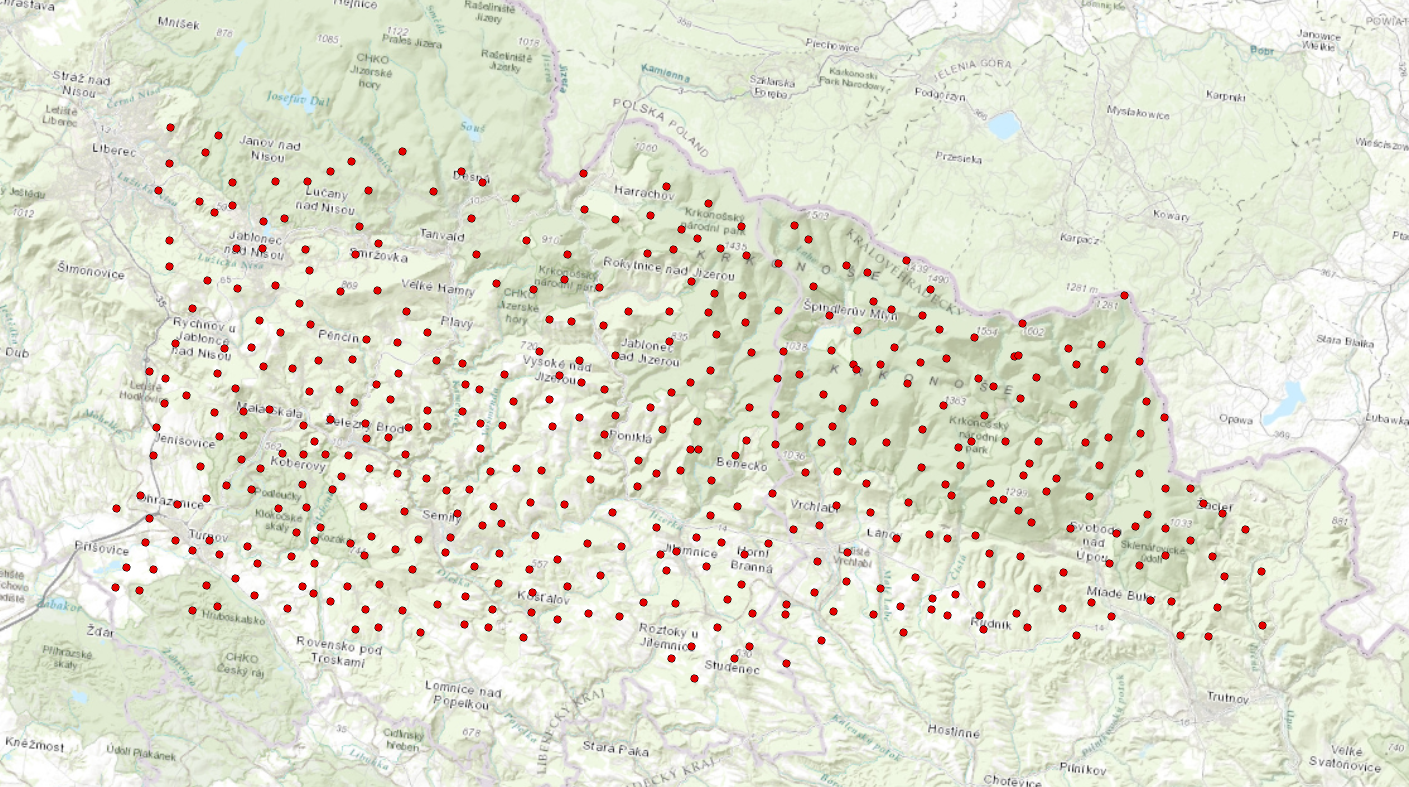
\includegraphics[width=15cm]{images/krkonose2.png} 
    \caption{Vymezení trigonometrických bodů na podkladové mapě.}
\end{figure}
\bigbreak
\par {\large\textbf{Případ 1: Oblast s malou vertikální členitostí} }
\par První zájmovou oblast zobrazuje obr. 11 v šesti oknech. Rozmístění bodů na podkladové mapě se nachází v okně (a), z čehož je zřejmé, že severní část oblasti je jen velmi málo členitá, vertikální členitost pak hlavně roste směrem na jihovýchod. Vygenerované vrstevnice s krokem 5 m, 10 m a 20 m jsou zobrazeny v oknech (b), (d), (f). Vrstevnice v rovinaté části odpovídají skutečnému průběhu terénu, s rostoucí nadmořskou výškou směrem na jihovýchod je pak správně naznačena změna členitosti s vyšší hustotou vrstevnic. Vrstevnice v nejjižnější části oblasti však zřejmě nejsou interpolovány správně, co je způsobeno tím, že zájmová oblast se nachází na okraji datasetu, pro který chybí další údaje o průběhu terénu. Je však zřejmé, že pro postačující výsledky lineární interpolace chybí množství bodů; jednotlivé segmenty tvořící vrstevnice jsou ostré, čímž dochází ke ztrátě informace o skutečné změně v tvaru reliéfu. 

\begin{figure}[H]

\begin{subfigure}{.475\linewidth}
\centering
  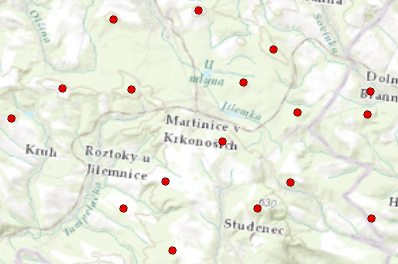
\includegraphics[width=7cm]{images/case1.png}
  \caption{zájmová oblast na podkladové mapě}
  \label{MLEDdet}
\end{subfigure}\hfill % <-- "\hfill"
\begin{subfigure}{.475\linewidth}
\centering
  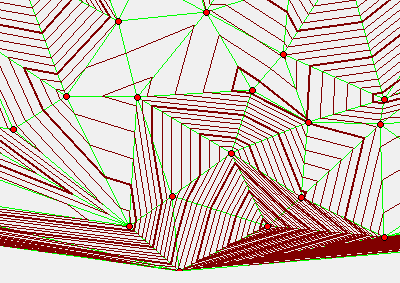
\includegraphics[width=7cm]{images/case1m5.png}
  \caption{vrstevnice s krokem 5 m}
  \label{energydetPSK}
\end{subfigure}\hfill
\medskip
\medskip
\begin{subfigure}{.475\linewidth}
\centering
  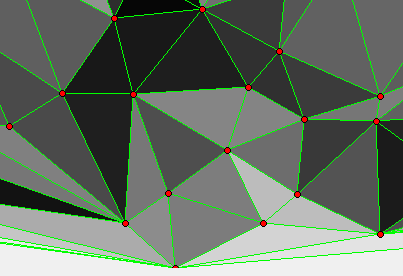
\includegraphics[width=7cm]{images/case1s.png}
  \caption{sklon terénu}
  \label{MLEDdet}
\end{subfigure}\hfill % <-- "\hfill"
\begin{subfigure}{.475\linewidth}
\centering
  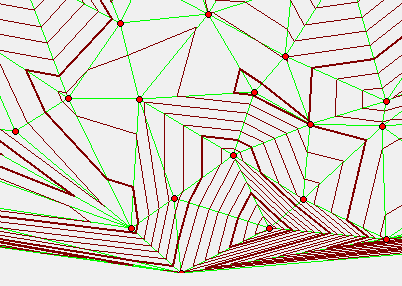
\includegraphics[width=7cm]{images/case1m.png}
  \caption{vrstevnice s krokem 10 m}
  \label{MLEDdet}
\end{subfigure}\hfill % <-- "\hfill"
\medskip
\begin{subfigure}{.475\linewidth}
\centering
  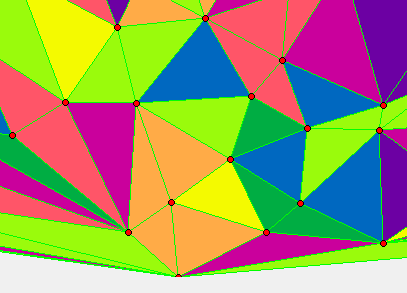
\includegraphics[width=7cm]{images/case1a.png}
  \caption{orientace terénu}
  \label{velcomp}
\end{subfigure}\hfill % <-- "\hfill"
\begin{subfigure}{.475\linewidth}
\centering
  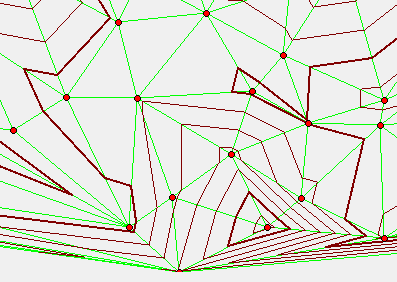
\includegraphics[width=7cm]{images/case1m20.png}
  \caption{vrstevnice s krokem 20 m}
  \label{estcomp}
\end{subfigure}

\caption{Zájmová oblast 1}
\label{fig:roc}
\end{figure}

\par Okno (c) znázorňující sklon svahů odpovídá vygenerovaným vrstevnicím: oblast s tmavými trojúhelníky naznačuje menší členitost, světlejší trojúhelníky naopak vyšší sklon svahu. Opět je důležité upozornit na světlé trojúhelníky v jižní části, které by podle takové analýzy znamenaly vysokou sklonitost terénu. Tento výsledek není správný a souvisí s okrajem analyzovaného území. Orientace svahů v okně (e) pak poukazuje na typy tvarů reliéfu: v jižní části je barevná paleta rozmanitější, což značí různou orientaci svahů kopce, resp. vrcholu, v severní části jsou pak barvy homogennější, protože na rovnějších oblastech nedochází k výrazné změně orientace svahů.
\bigbreak

\par {\large\textbf{Případ 2: Oblast s velkou vertikální členitostí} }
\par Druhá zájmová oblast (obr. 12) se nachází v nejvyšších částech Krkonoš a je charakterizována velkým počtem hřbetů, vrcholů a údolí. Podle vygenerovaných vrstevnic v oknech (b), (d) a (f) je však patrné, že tato oblast nebyla z hlediska výškopisu popsána správně. I když hustota vrstevnic potvrzuje prudkou změnu výškových poměrů, vzhledem k malému počtu bodů vrstevnice nenásledují průběh hřbetů a zcela ignorují většinu údolí. Příčinou je také rozmístění bodů, které v údolích a nižších částech území úplně chybějí a tyto reliéfní tvary tak nemohou být zkonstruovány. Rozmístění bodů také ovlivňuje velikost trojúhelníků, přičemž opět platí, že velké trojúhelníky nemusí dostatečně charakterizovat tvar terénu. Protože je tato oblast opět na okraji datasetu, došlo k nesprávné interpolaci okraje oblasti stejně jako v případě 1.

\begin{figure}[H]

\begin{subfigure}{.475\linewidth}
\centering
  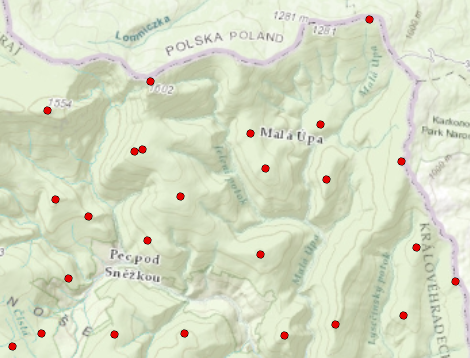
\includegraphics[width=7cm]{images/case2.png}
  \caption{zájmová oblast na podkladové mapě}
  \label{MLEDdet}
\end{subfigure}\hfill % <-- "\hfill"
\begin{subfigure}{.475\linewidth}
\centering
  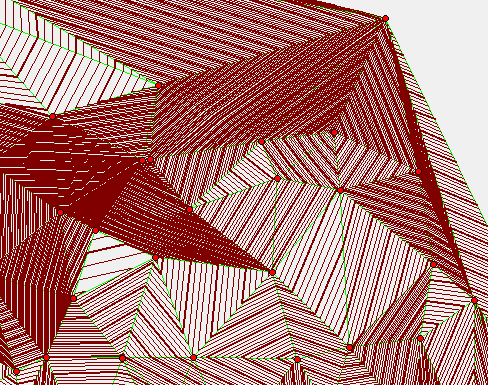
\includegraphics[width=7cm]{images/case2m5.png}
  \caption{vrstevnice s krokem 5 m}
  \label{energydetPSK}
\end{subfigure}\hfill
\medskip
\medskip
\begin{subfigure}{.475\linewidth}
\centering
  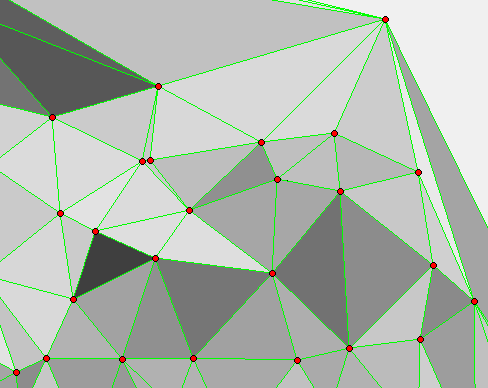
\includegraphics[width=7cm]{images/case2s.png}
  \caption{sklon terénu}
  \label{MLEDdet}
\end{subfigure}\hfill % <-- "\hfill"
\begin{subfigure}{.475\linewidth}
\centering
  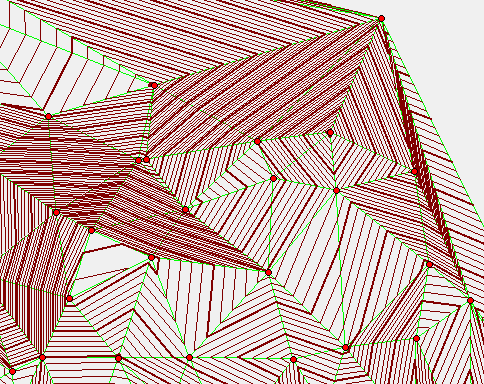
\includegraphics[width=7cm]{images/case2m.png}
  \caption{vrstevnice s krokem 10 m}
  \label{MLEDdet}
\end{subfigure}\hfill % <-- "\hfill"
\medskip
\begin{subfigure}{.475\linewidth}
\centering
  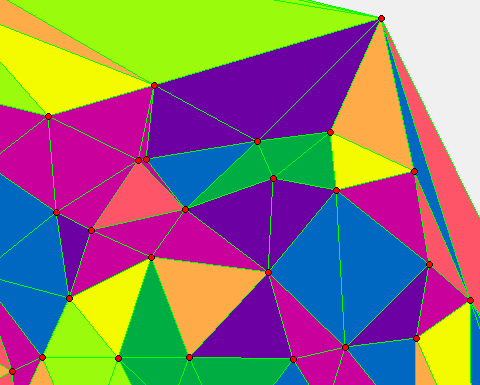
\includegraphics[width=7cm]{images/case2a.png}
  \caption{orientace terénu}
  \label{velcomp}
\end{subfigure}\hfill % <-- "\hfill"
\begin{subfigure}{.475\linewidth}
\centering
  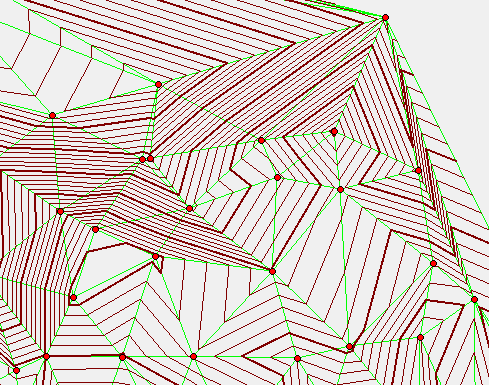
\includegraphics[width=7cm]{images/case2m20.png}
  \caption{vrstevnice s krokem 20 m}
  \label{estcomp}
\end{subfigure}

\caption{Zájmová oblast 2}
\label{fig:roc}
\end{figure}

\par Další zajímavou chybu v modelu odhaluje okno (c) se sklonem terénu, kde je možné pozorovat tmavý trojúhelník v západní části oblasti uprostřed prudkých svahů, což naznačuje rovinatou oblast. Není tomu tak, v skutečnosti vrcholy tohoto trojúhelníku tvoří vrcholy s podobnými nadmořskými výškami a zcela opomíjejí údolí, nad kterým se vypínají. Světlost většiny trojúhelníků však potvrzuje, že se jedná o horskou oblast. Orientaci terénu v okně (e) ovlivňuje nadmořská výška nejvyššího z vrcholů trojúhelníku, a tedy na některých místech, kde dochází k opomenutí reliefních tvarů, je orientace terénu vůči světovým stranám určena nesprávně.
\bigbreak
\par {\large\textbf{Případ 3: oblast s hřebenem a údolími} }
\par Poslední ukázka se věnuje oblasti v severozápadní části analyzovaných dat. Detail oblasti i s grafickými výsledky jsou k dispozici na Obrázku 13. 

\begin{figure}[H]

\begin{subfigure}{.475\linewidth}
\centering
  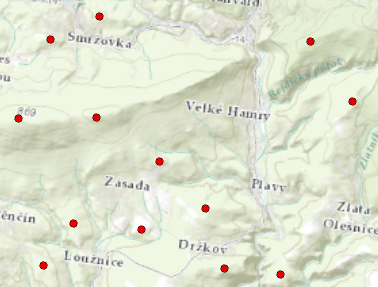
\includegraphics[width=7cm]{images/case3.png}
  \caption{zájmová oblast na podkladové mapě}
  \label{MLEDdet}
\end{subfigure}\hfill % <-- "\hfill"
\begin{subfigure}{.475\linewidth}
\centering
  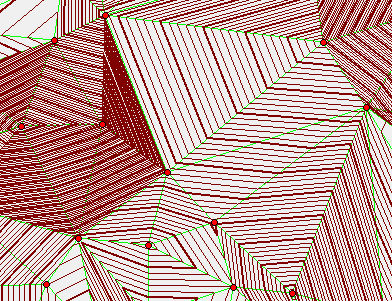
\includegraphics[width=7cm]{images/case3m5.png}
  \caption{vrstevnice s krokem 5 m}
  \label{energydetPSK}
\end{subfigure}\hfill
\medskip
\medskip
\begin{subfigure}{.475\linewidth}
\centering
  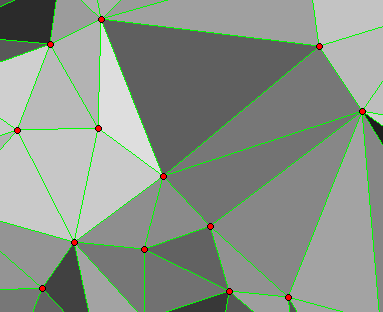
\includegraphics[width=7cm]{images/case3s.png}
  \caption{sklon terénu}
  \label{MLEDdet}
\end{subfigure}\hfill % <-- "\hfill"
\begin{subfigure}{.475\linewidth}
\centering
  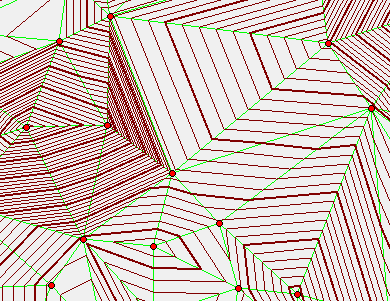
\includegraphics[width=7cm]{images/case3m.png}
  \caption{vrstevnice s krokem 10 m}
  \label{MLEDdet}
\end{subfigure}\hfill % <-- "\hfill"
\medskip
\begin{subfigure}{.475\linewidth}
\centering
  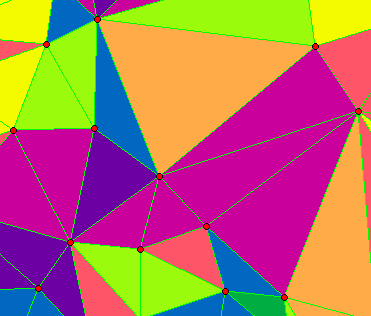
\includegraphics[width=7cm]{images/case3a.png}
  \caption{orientace terénu}
  \label{velcomp}
\end{subfigure}\hfill % <-- "\hfill"
\begin{subfigure}{.475\linewidth}
\centering
  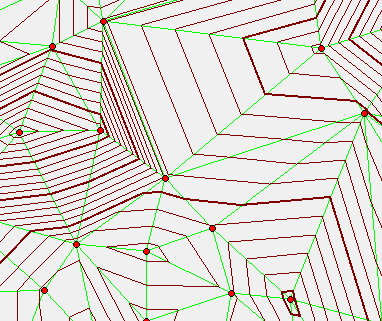
\includegraphics[width=7cm]{images/case3m20.png}
  \caption{vrstevnice s krokem 20 m}
  \label{estcomp}
\end{subfigure}

\caption{Zájmová oblast 3}
\label{fig:roc}
\end{figure}

\par Tato oblast může při grafickém znázornění vrstevnic na první pohled rychle zaujmout: určité trojúhelníky hustěji vyplněny vrstevnicemi díky rychlému nárůstu výšky. Pokud výsledek srovnáme s realitou, tak je patrné, že vzniklá triangulace v okolí dvou bodů na hřebenu (na obrázku (a) se nacházejí na v západní části) proběhla až na malé odlišnosti dobře. Ovšem tento hřeben pokračuje směrem na východ (severovýchod), což výsledek vizualizovaných vrstevnic nerespektuje. Tato skutečnost, jak již bylo zmíněno, vyplývá z faktu, že algoritmus, který je použitý pro výpočet triangulace, nerespektuje žádné překážky jako vodní toky nebo silnice. Hřeben by měl pokračovat dál na východ, který se mírně svažuje a následně je přerušen údolím. Na druhý pohled je však z výsledků vygenerovaných vrstevnic vidět jakýsi náznak údolí, které ovšem prochází středem sledované zájmové oblasti. Lze tedy říci, že pokud bychom měli k dispozici více bodů z terénu, nebo by bylo do výpočtu zahrnuto respektování bariér (řeky,\dots) výsledek triangulace by více odpovídal skutečnosti. Pokud se budeme soustředit na expozici svahu v okolí těchto bodů (e) zjistíme, že výsledek odpovídá skutečnosti a lze tedy potvrdit, že implementovaný algoritmus pro analýzu orientace svahu pracuje správně.
\par Uprostřed jižní části výřezu se nachází bod, který dle výsledné triangulace a i vzhledem k realitě reprezentuje vrchol kopce. Ovšem ve skutečnosti se směrem na jih/jihovýchod nachází rovina, kterou algoritmus nemá šanci (vzhledem k datům) rozpoznat. Opět lze tedy konstatovat, že nad analyzovanými daty je zanedbaná důležitá informace o průběhu terénu. V této části zájmového území neodpovídá analýza sklonu ani orientace terénu skutečnosti. Pokud bychom ovšem nahlíželi na území jen z hlediska výšky, pak je výsledná analýza provedená správně.

\bigbreak
\par {\large\textbf{Shrnutí} }
\par Implementované metody pro konstrukci a analýzu DMT byly otestovány na členitém reliéfu Krkonoš s nereprezentativním vzorkem dat. I přestože byly určité části území popsány z hlediska výškopisu, svažitosti a orientace svahů vůči světovým stranám správně, není možné ohodnotit celkový výsledek analýzy vytvořeného modelu kladně. Jako hlavní příčiny byly identifikovány následující skutečnosti:
\begin{itemize}
    \item nedostatečný počet bodů v datasetu, a tedy menší počet trojúhelníků na místech, kde se tvar reliéfu mění intenzivněji,
    \item nevhodné rozmístění bodů, které se nacházejí téměř výhradně na vrcholech pohoří a na níže položených místech území zcela chybějí,
    \item využití lineární interpolace, která není pro náročnější terén vhodná a je vhodné ji doplnit jinými technikami/metodami.
\end{itemize}

\par Bylo by vhodné provést konstrukci a analýzu DMT nad jiným datasetem, který by zohledňoval výše popsané nedostatky.

